\pdfminorversion=4 % For adobe reader to work

% The SP beamer class has the options electronics, notopline and swedish
%\documentclass[aspectratio=169]{beamer}
%\documentclass[aspectratio=169,notopline]{beamer}
%\documentclass[aspectratio=169,swedish]{beamer}
\documentclass[aspectratio=169,electronics,notopline]{beamer}
%\documentclass[aspectratio=169,electronics,swedish]{beamer}

%\usepackage[utf8]{inputenc}
\usepackage[T1]{fontenc}
\usepackage{tikz}
\usepackage{graphicx} 

\usetheme{sp}

\title{The SP RC Car}
\author[Euclid]{Benjamin Vedder\\
\texttt{benjamin.vedder@sp.se}}
%\date{\today}
\date{2016-07-06, Darmstadt}

\begin{document}

\spStartFrame
\maketitle

%\AtBeginSection[]
%{
%\begin{frame}<beamer>{Table of Contents}
%\tableofcontents[currentsection,currentsubsection, 
%    hideothersubsections, 
%    sectionstyle=show/shaded,
%]
%\end{frame}
%}

\section{Overview}

\begin{frame}{The SP RC Car}
\begin{center}
	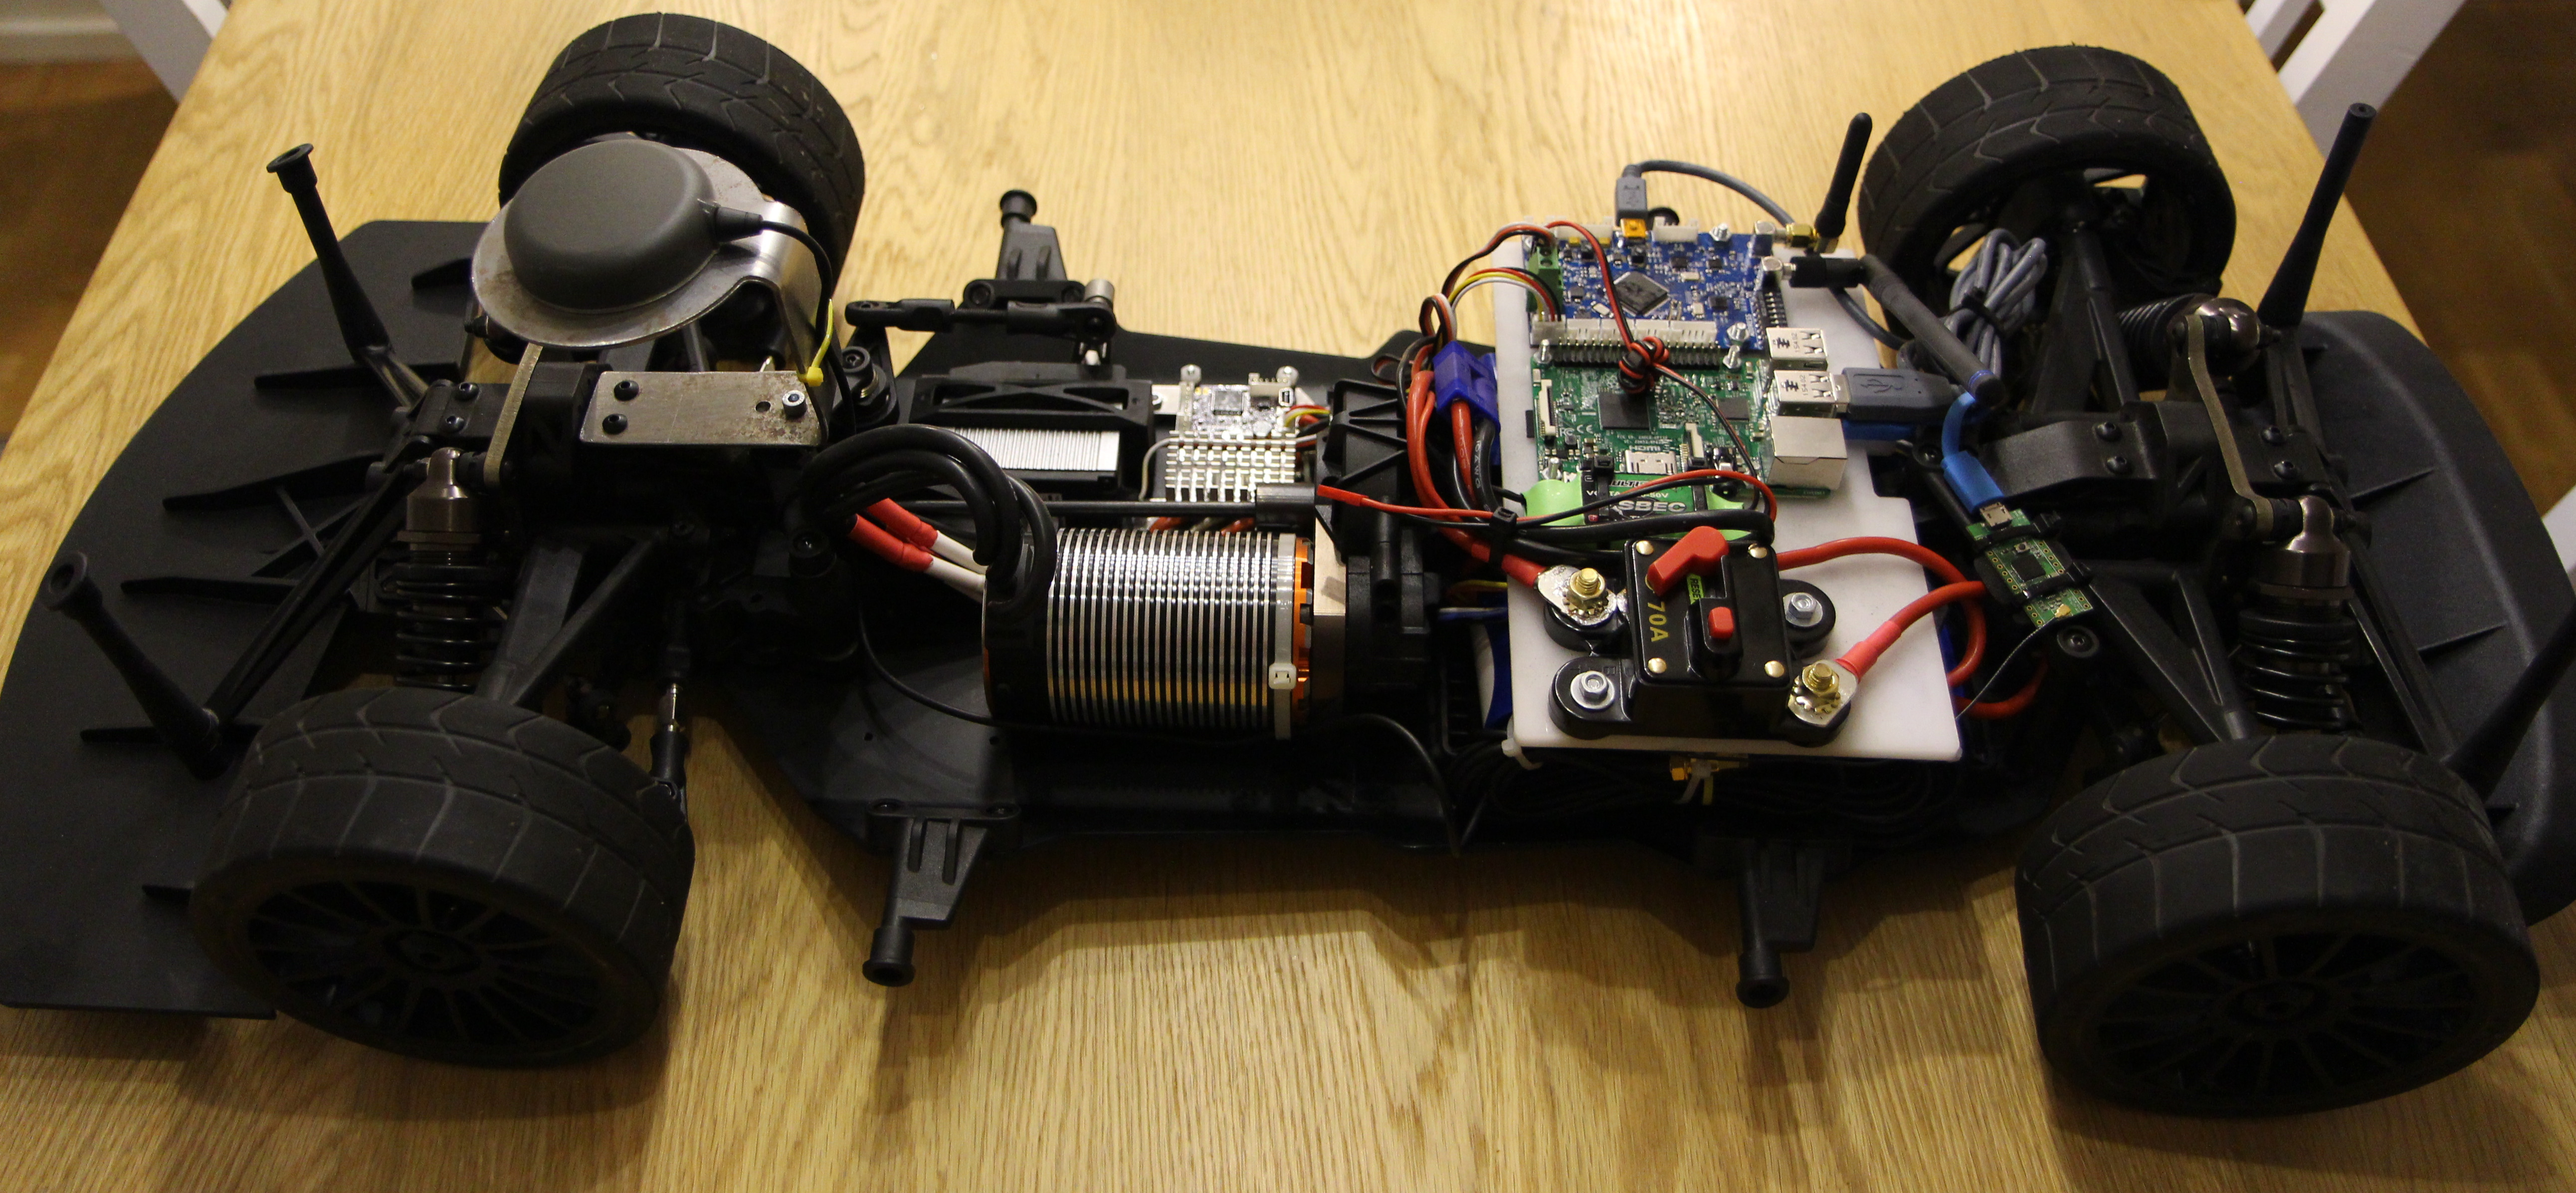
\includegraphics[width=12cm]{Figures/car_2.jpg}
\end{center}
\end{frame}

\begin{frame} 
\frametitle{The SP RC Car}
\framesubtitle{Overview}
\begin{columns}[c]
\column{.5\textwidth}
\begin{itemize}
\item Positioning:
	\begin{itemize}
	\item IMU (Accelerometer, Gyroscope,  Magnetometer).
	\item RTK GPS.
	\item Odometry.
	\end{itemize}
\item Speed from <1 Km/h to 80 Km/h
\item Autopilot.
\item Custom user interface.
\begin{itemize}
\item Visualization, remote control, configuration, communication.
\item RTK correction data from different possible sources.
\end{itemize}
\item Fully open source.
\end{itemize}
\column{.5\textwidth}
\begin{center}
	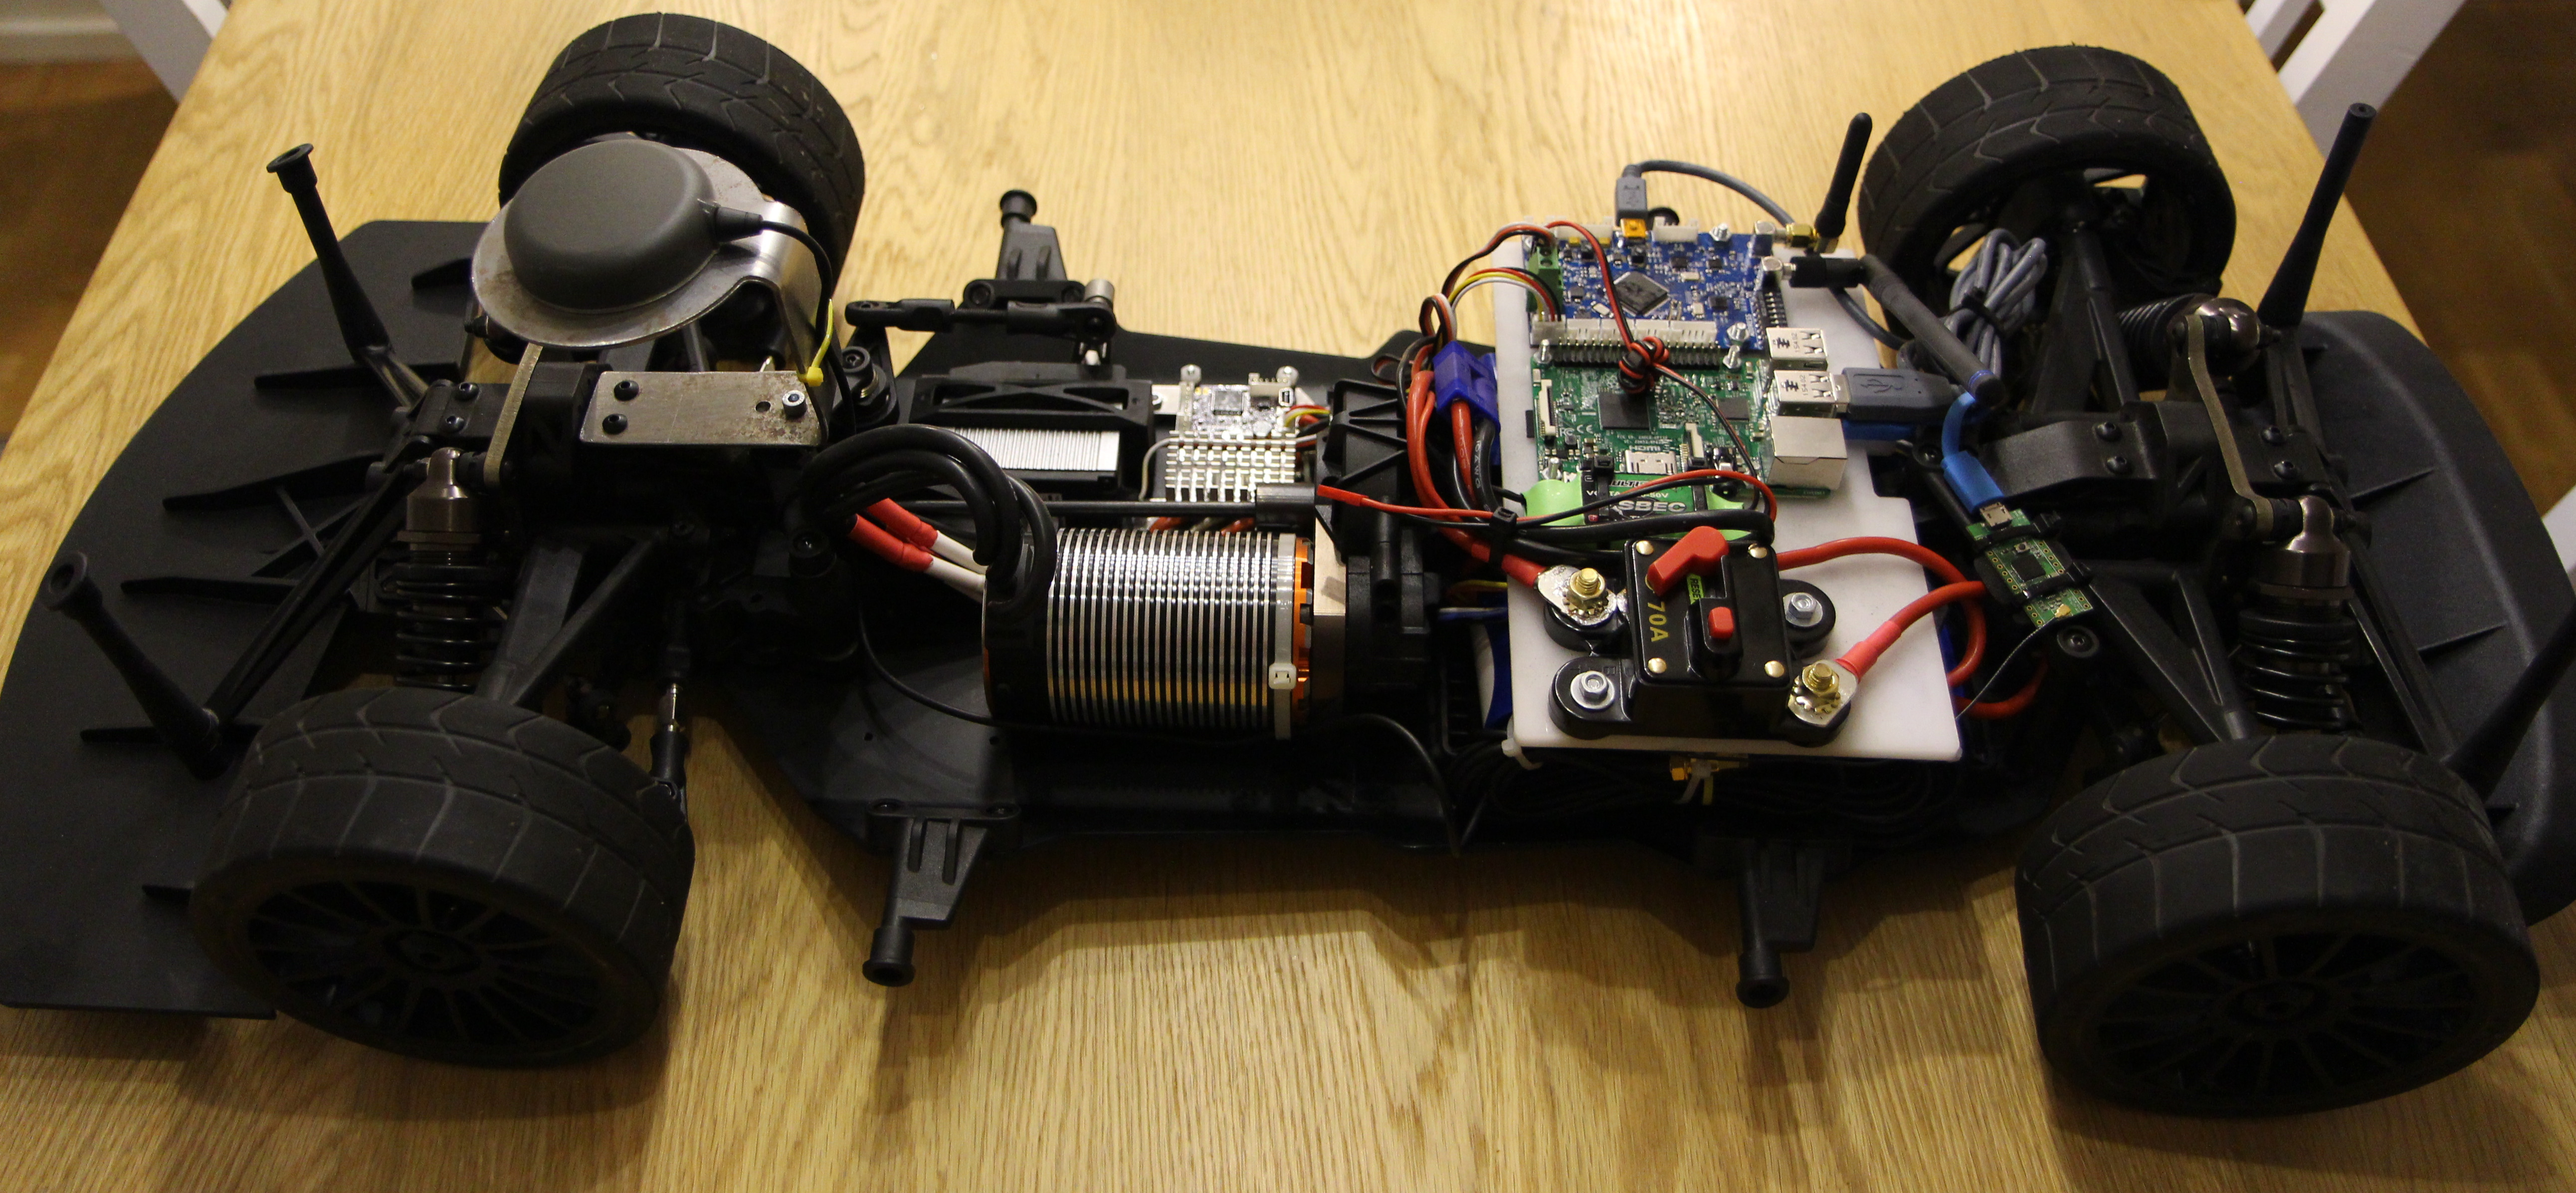
\includegraphics[width=6cm]{Figures/car_2.jpg}
\end{center}
\end{columns}
\end{frame}

\begin{frame}[c]
\frametitle{The SP RC Car}
\framesubtitle{RTK GPS for accurate positioning}
\begin{center}
	\begin{columns}[c]
		\column{.5\textwidth}
			\centering
			\textbf{SPP}\\
			\vspace{0.2cm}
			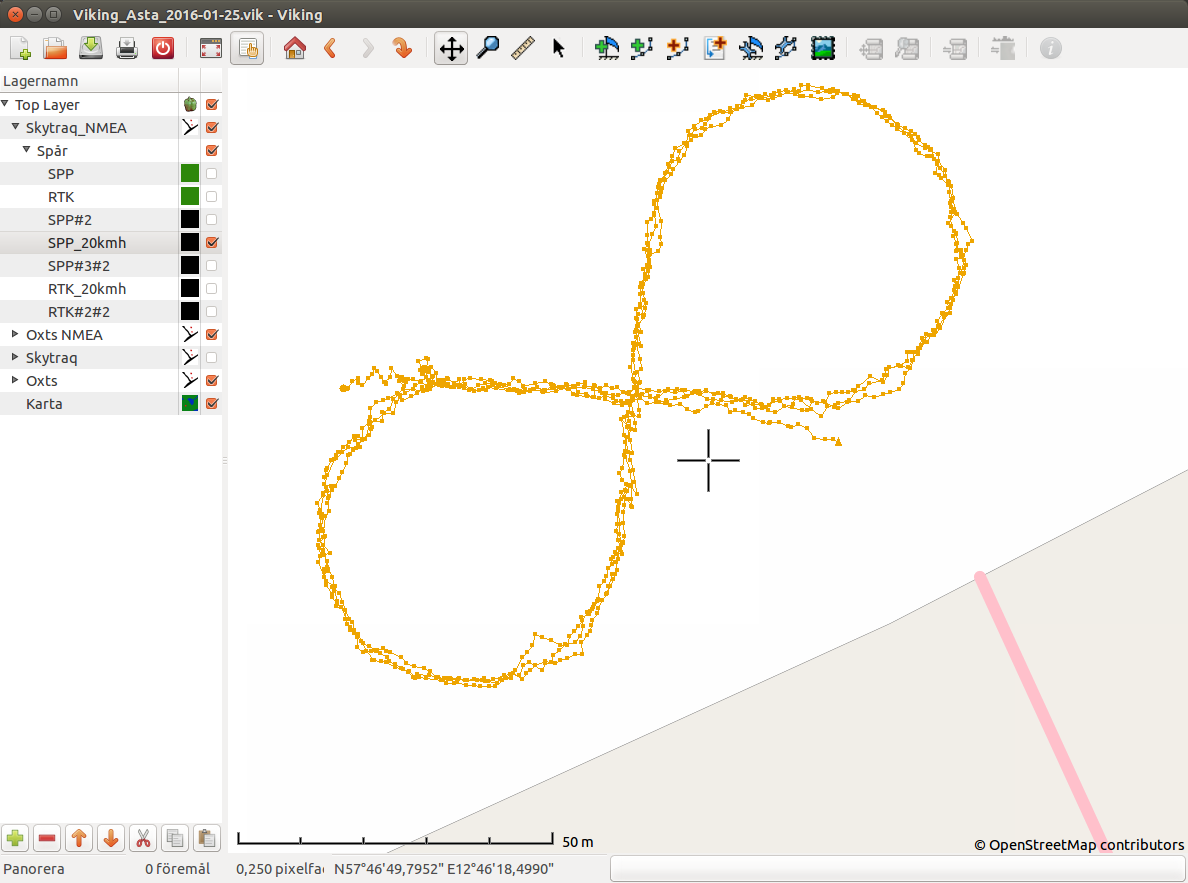
\includegraphics[width=65mm]{Figures/viking_dyn_spp.png}
		\column{.5\textwidth}
			\centering
			\textbf{RTK}\\
			\vspace{0.2cm}
			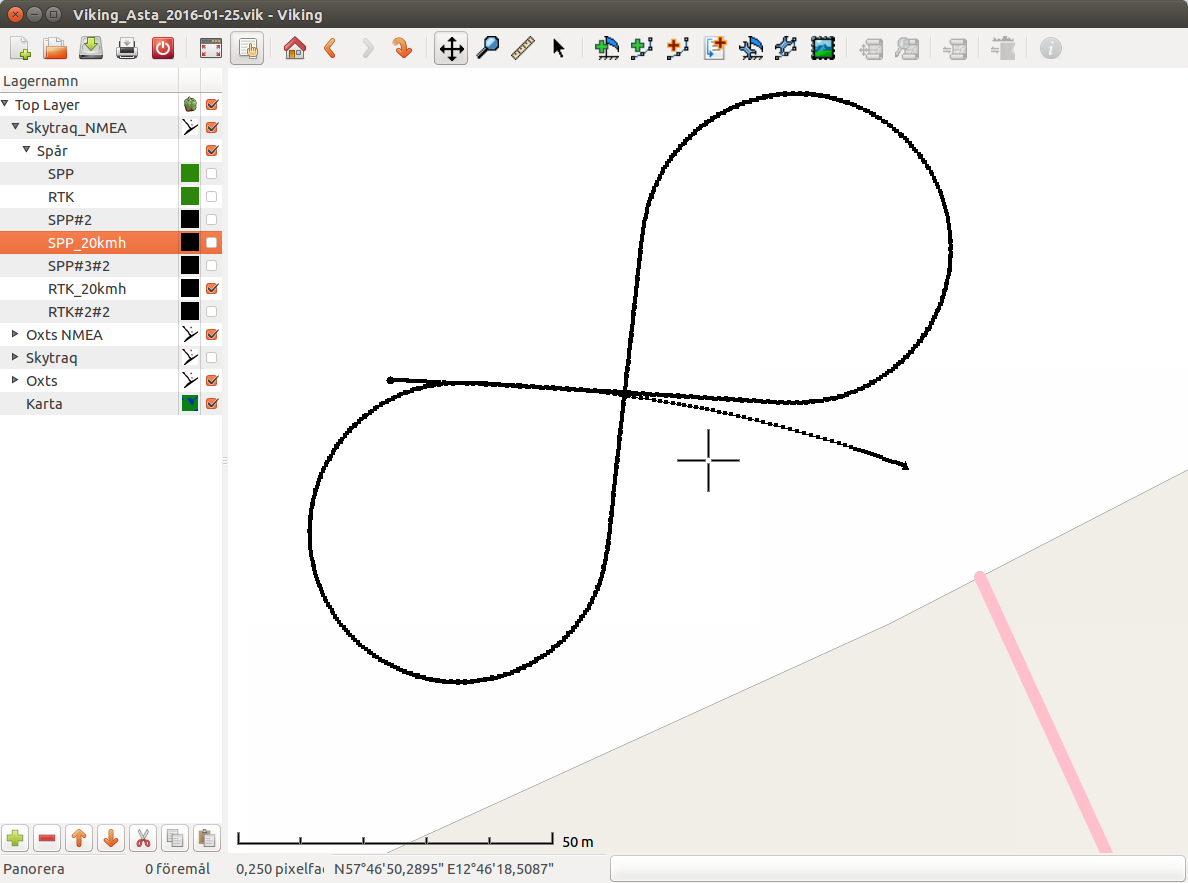
\includegraphics[width=65mm]{Figures/viking_dyn_rtk.png}
	\end{columns}
\end{center}
\end{frame}

\begin{frame} 
\frametitle{The SP RC Car}
\framesubtitle{Hardware Block Diagram}
\begin{center}
	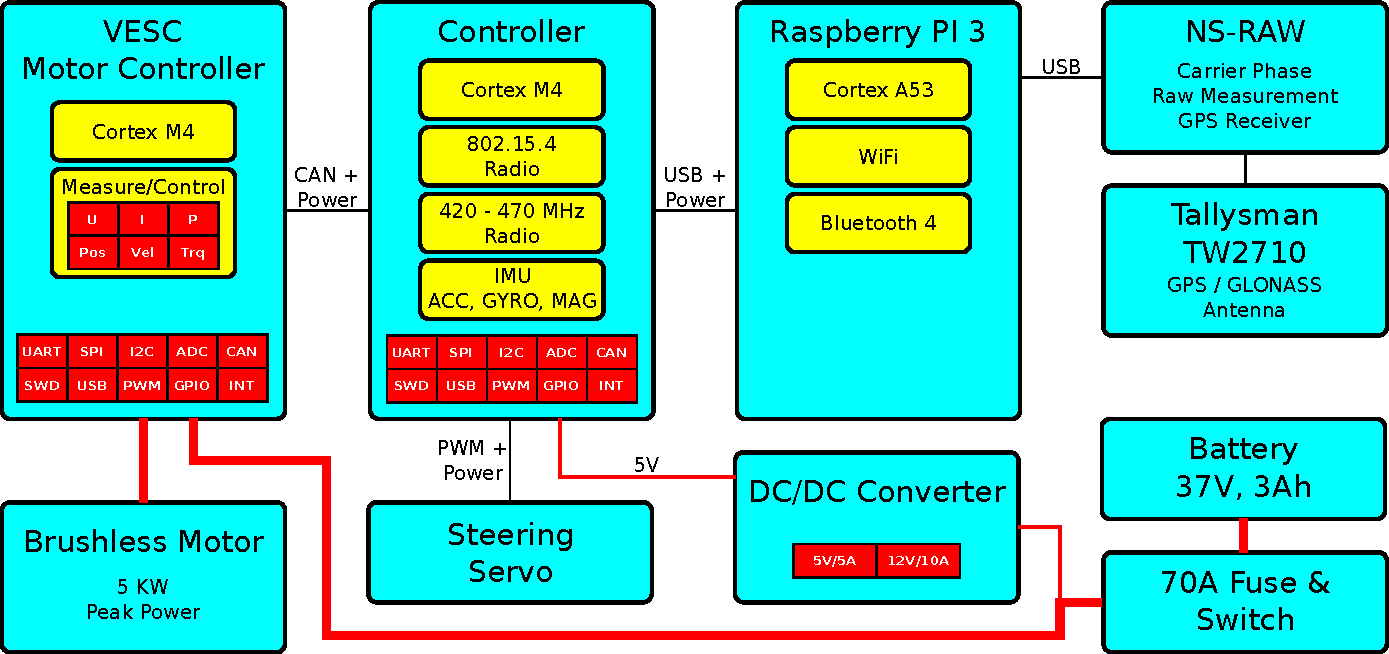
\includegraphics[width=12cm]{Figures/block_diagram.pdf}
\end{center}
\end{frame}

\begin{frame} 
\frametitle{The SP RC Car}
\framesubtitle{Hardware Locations}
\begin{center}
	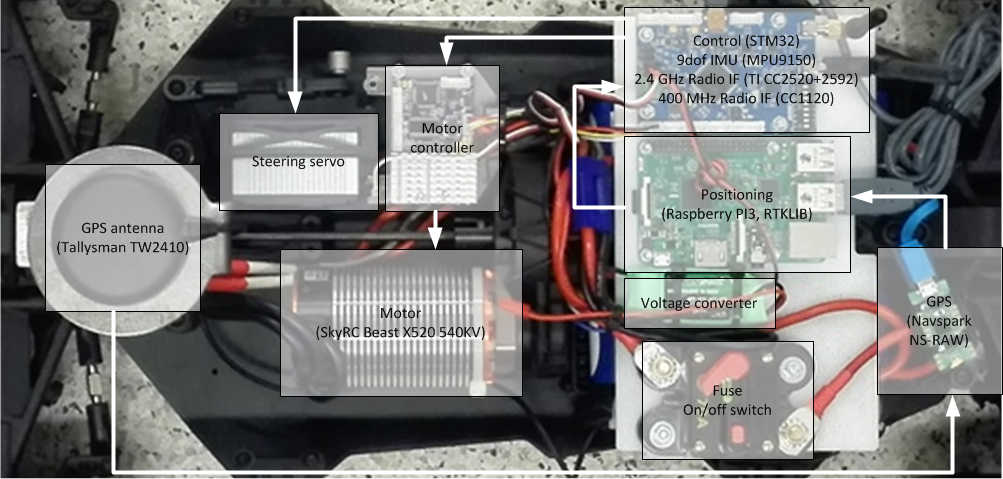
\includegraphics[width=12cm]{Figures/car_overview.png}
\end{center}
\end{frame}

\begin{frame}
\frametitle{The SP RC Car}
\framesubtitle{VESC Motor Controller}
\begin{columns}
\column{.5\textwidth}
\begin{itemize}
\item Benjamins open source and open hardware spare time project developed during the past 4 years.
\item 20 000+ lines of C code in 100+ files.
\end{itemize}
\column{.5\textwidth}
\begin{center}
\begin{itemize}
\item 14 threads + interrupts and DMA.
\item Cont power: 2000W
\item Peak power: over 5000W
\item Size: 40mm x 60mm and 40g weight.
\end{itemize}
\end{center}
\end{columns}
\begin{center}
\vspace{-3mm}
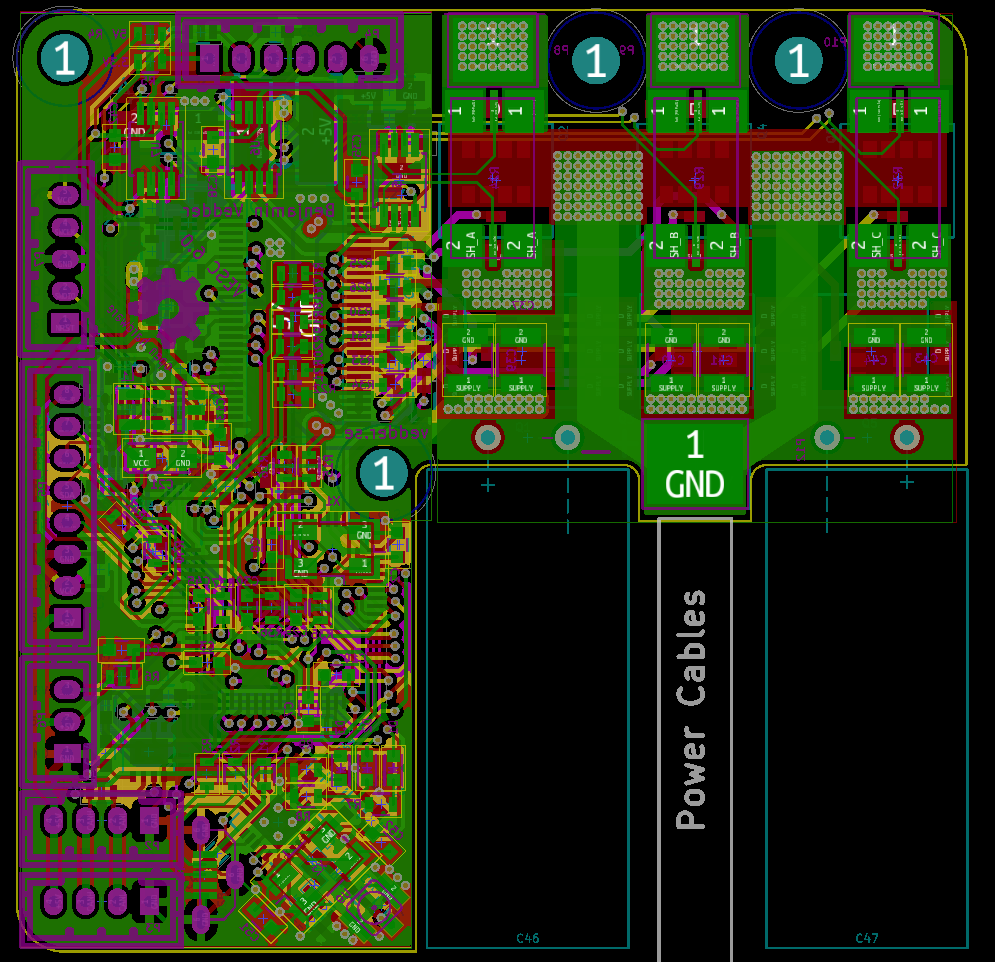
\includegraphics[height=40mm]{Figures/VESC_6.png} \hspace{5mm}
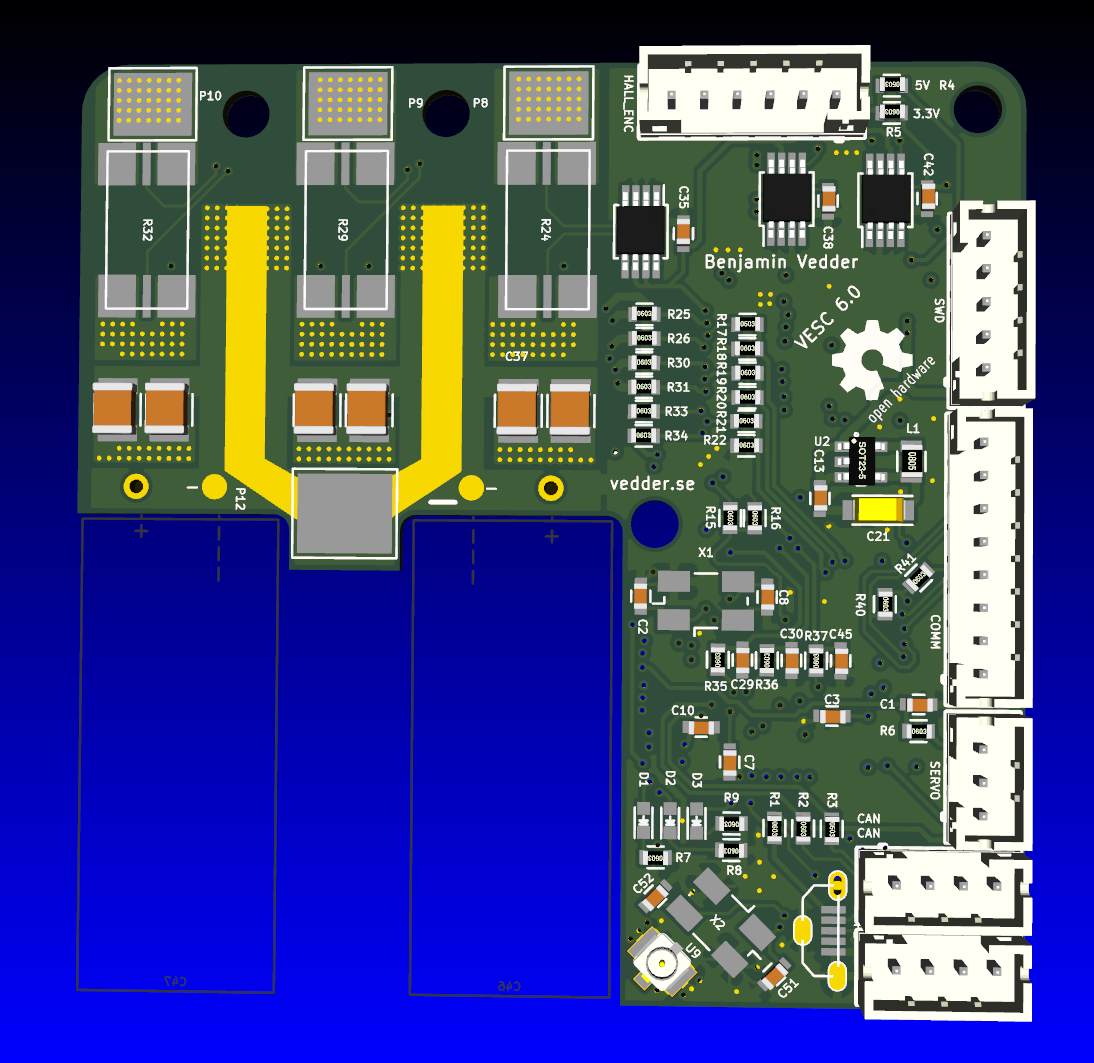
\includegraphics[height=40mm]{Figures/VESC_6_F.png} \hspace{5mm}
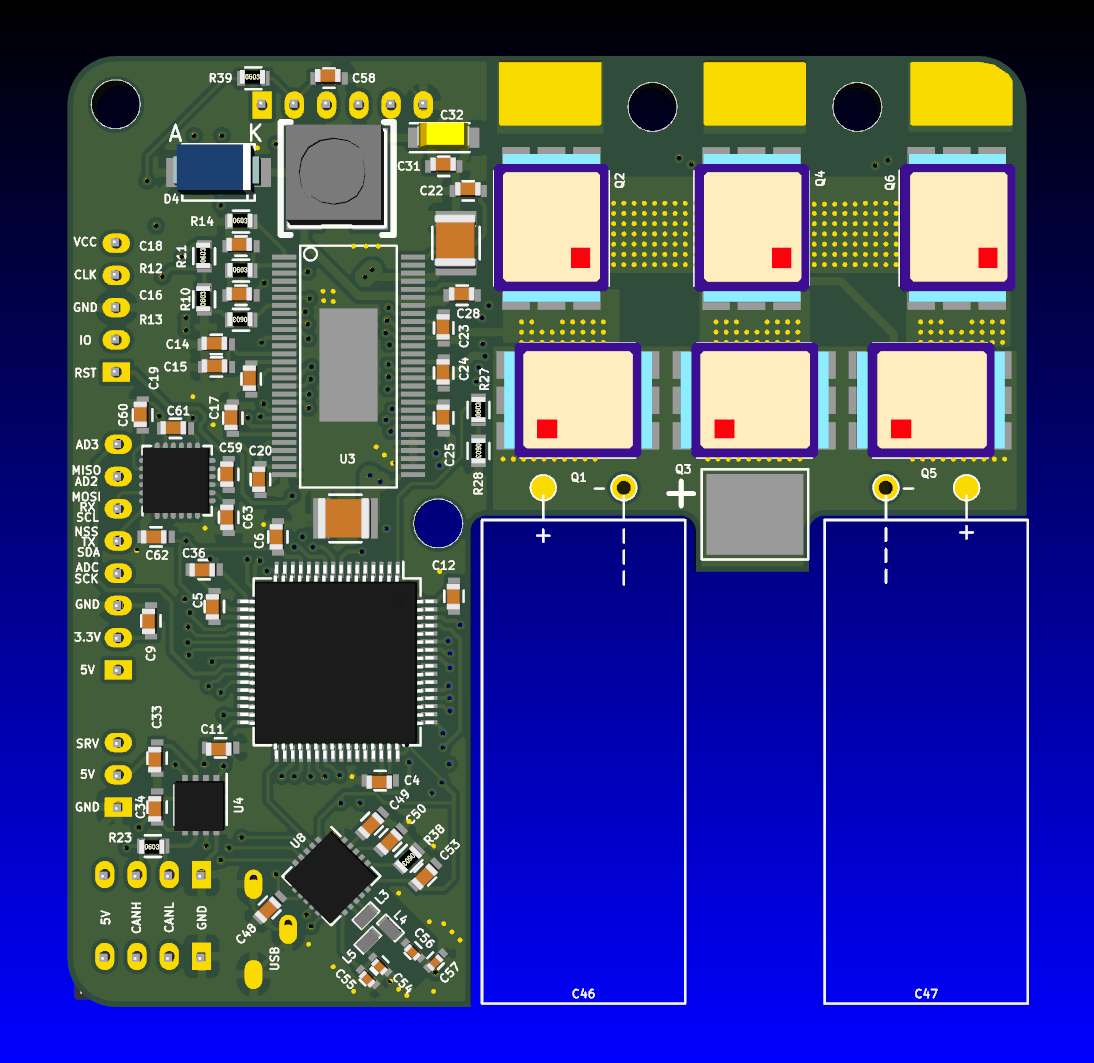
\includegraphics[height=40mm]{Figures/VESC_6_B.png}
\end{center}
\end{frame}

\begin{frame}
\frametitle{The SP RC Car}
\framesubtitle{VESC - BLDC Tool GUI}
\begin{center}
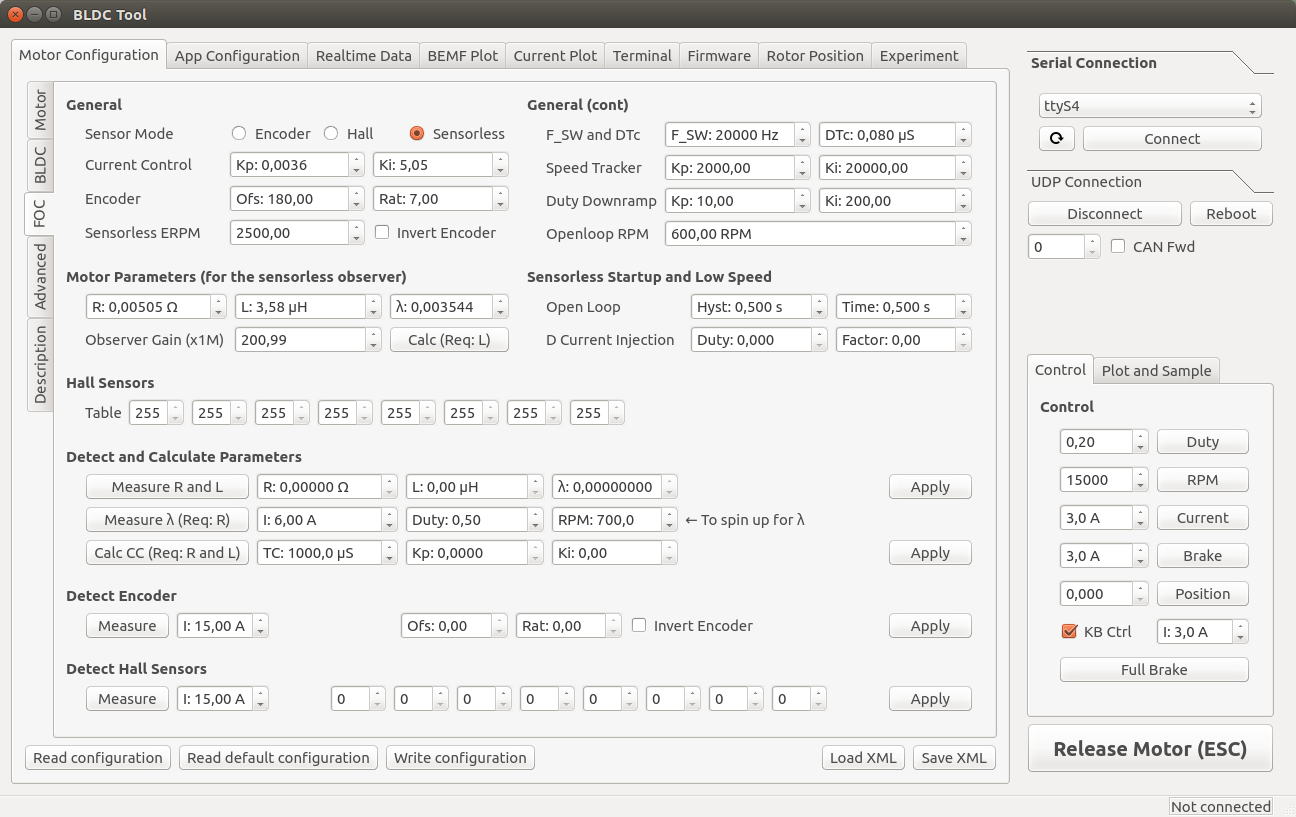
\includegraphics[height=65mm]{Figures/BLDC_Tool_FOC.png}
\end{center}
\end{frame}

\begin{frame} 
\frametitle{The SP RC Car}
\framesubtitle{Main Controller - front}
\begin{center}
	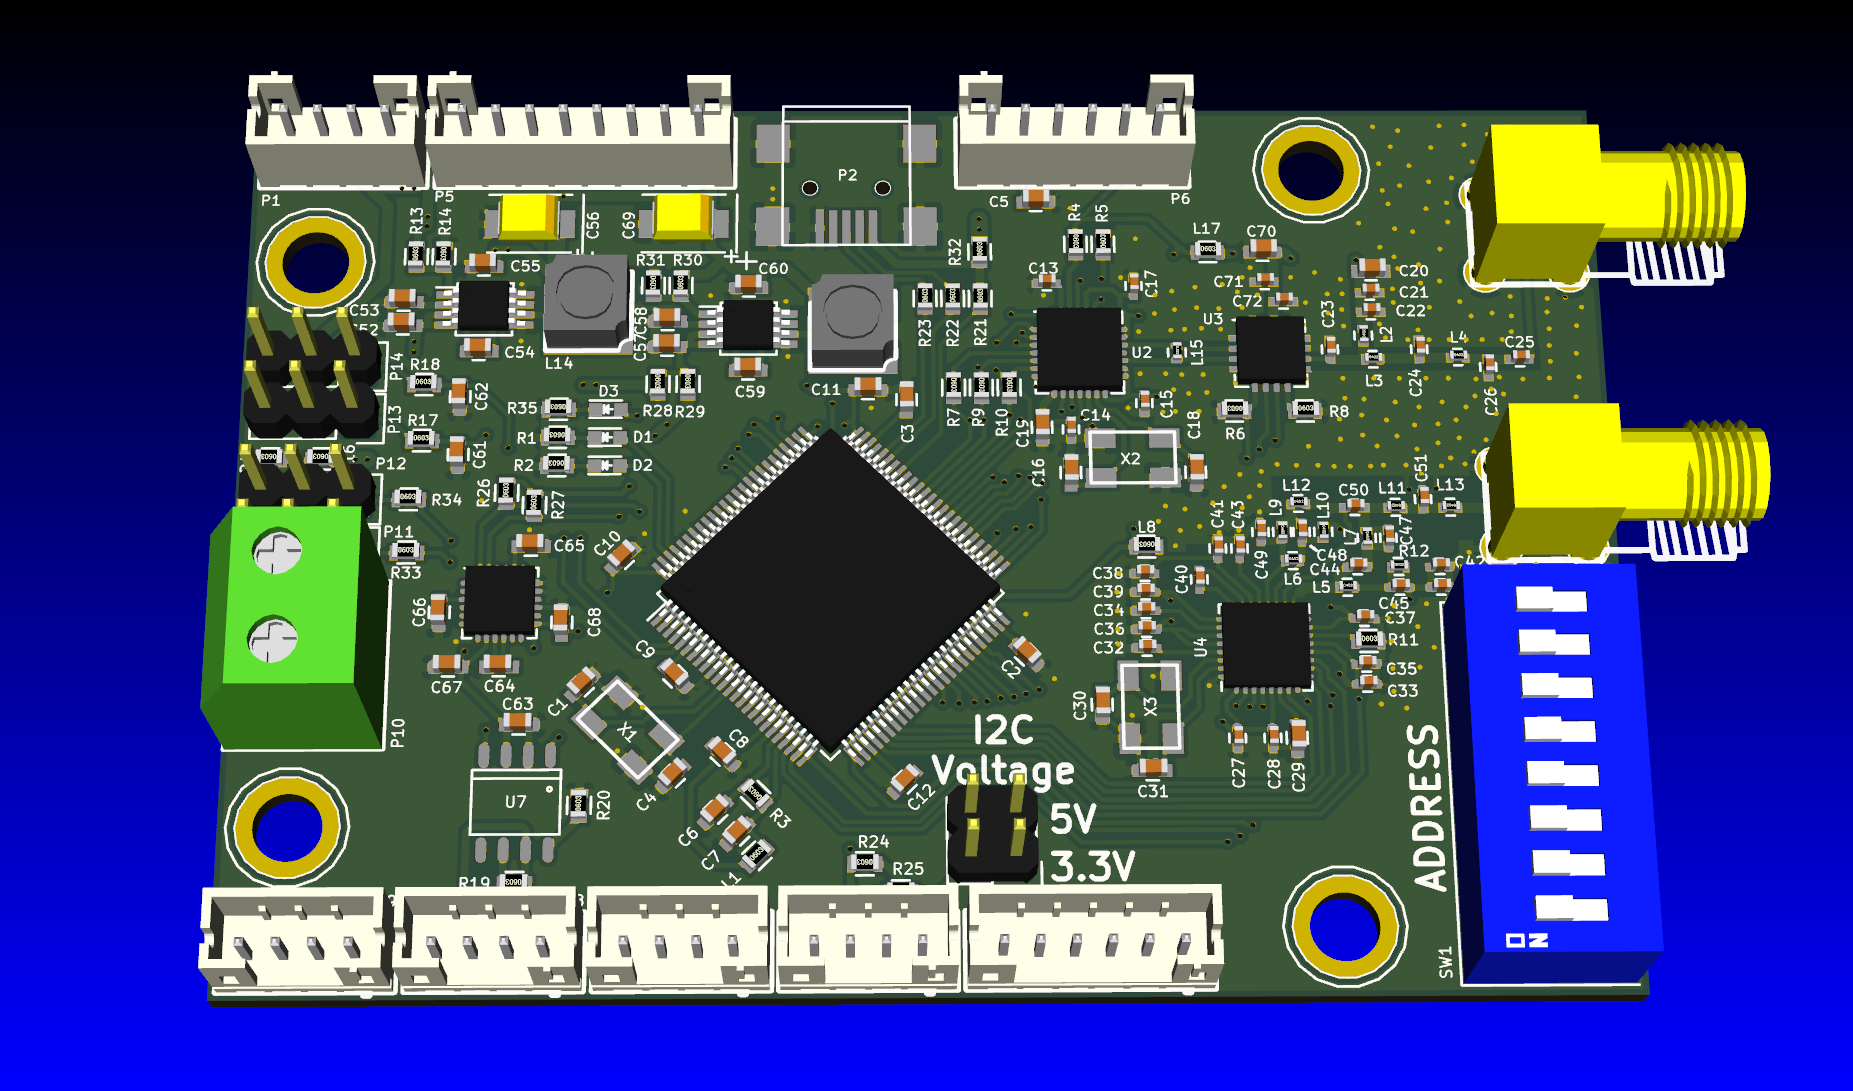
\includegraphics[width=10cm]{Figures/controller_front.png}
\end{center}
\end{frame}

\begin{frame} 
\frametitle{The SP RC Car}
\framesubtitle{Controller - back}
\begin{center}
	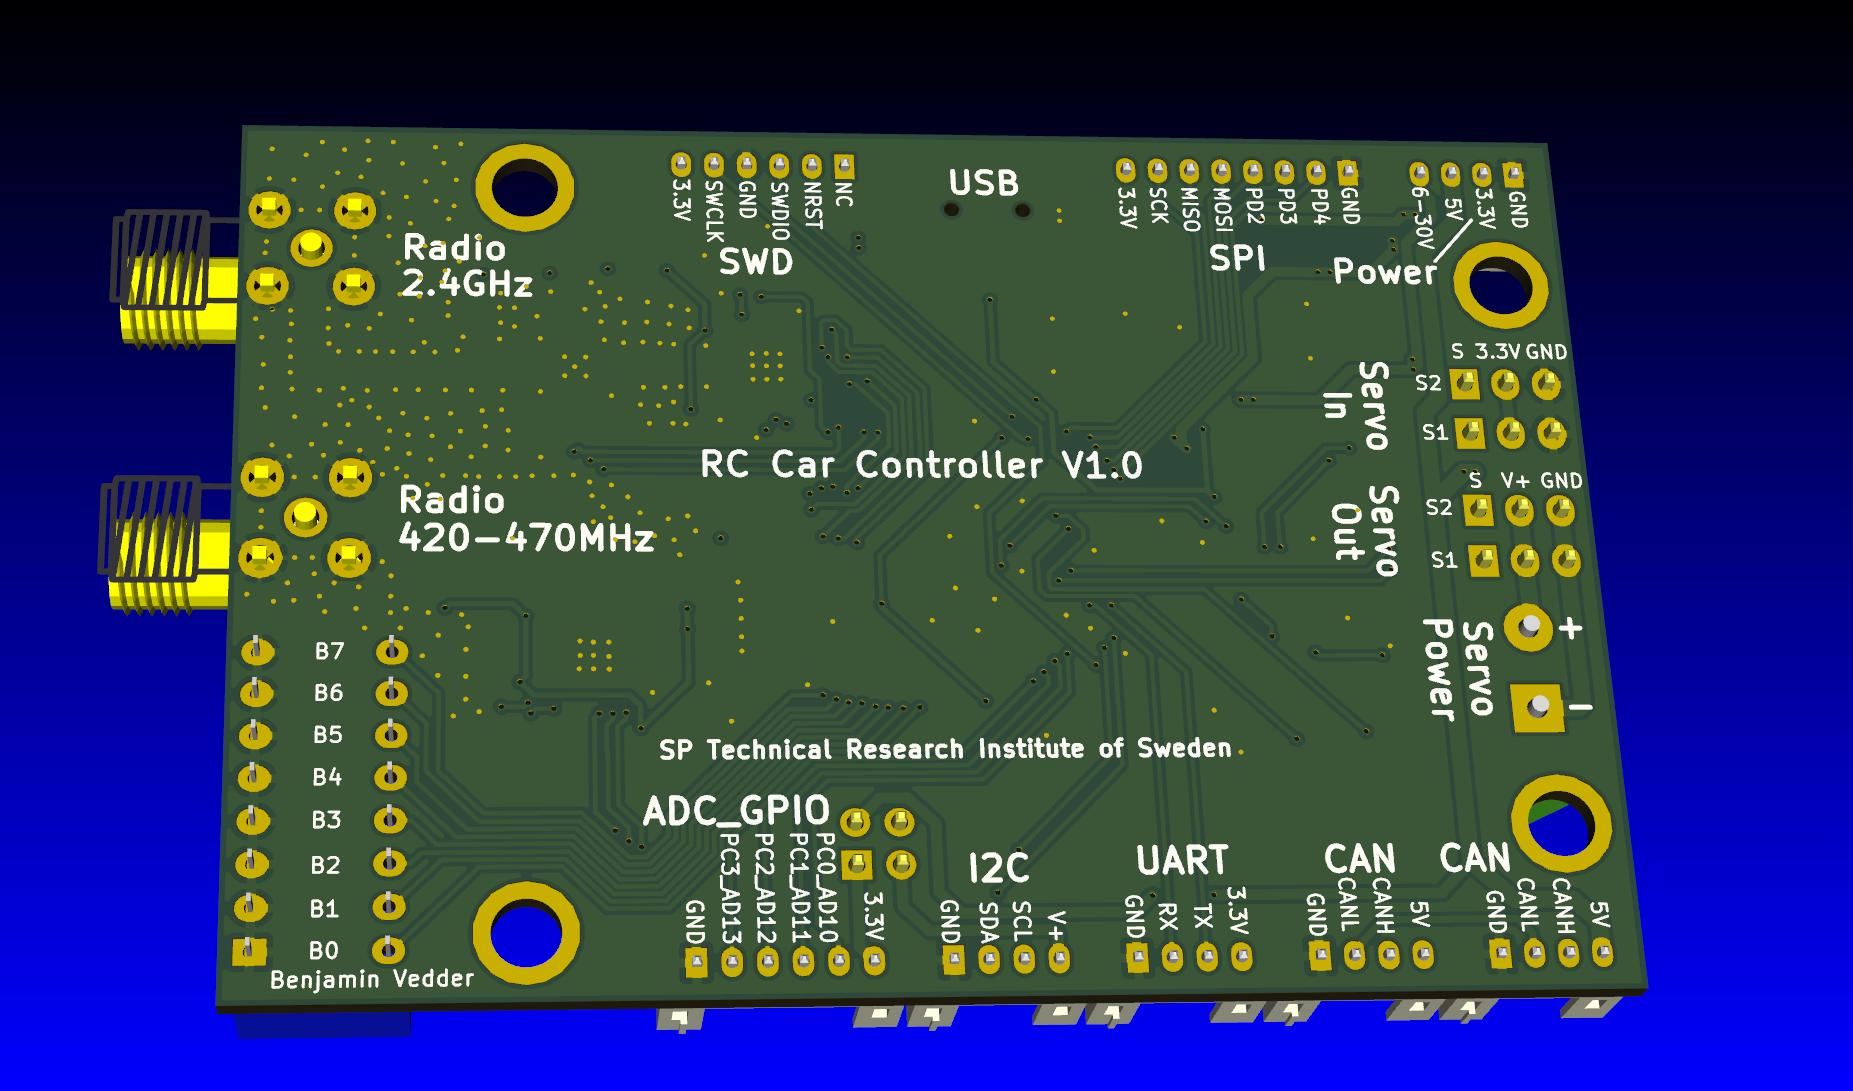
\includegraphics[width=10cm]{Figures/controller_back.png}
\end{center}
\end{frame}

\begin{frame} 
\frametitle{The SP RC Car}
\framesubtitle{RC Car Tool - Main Page}
\begin{center}
	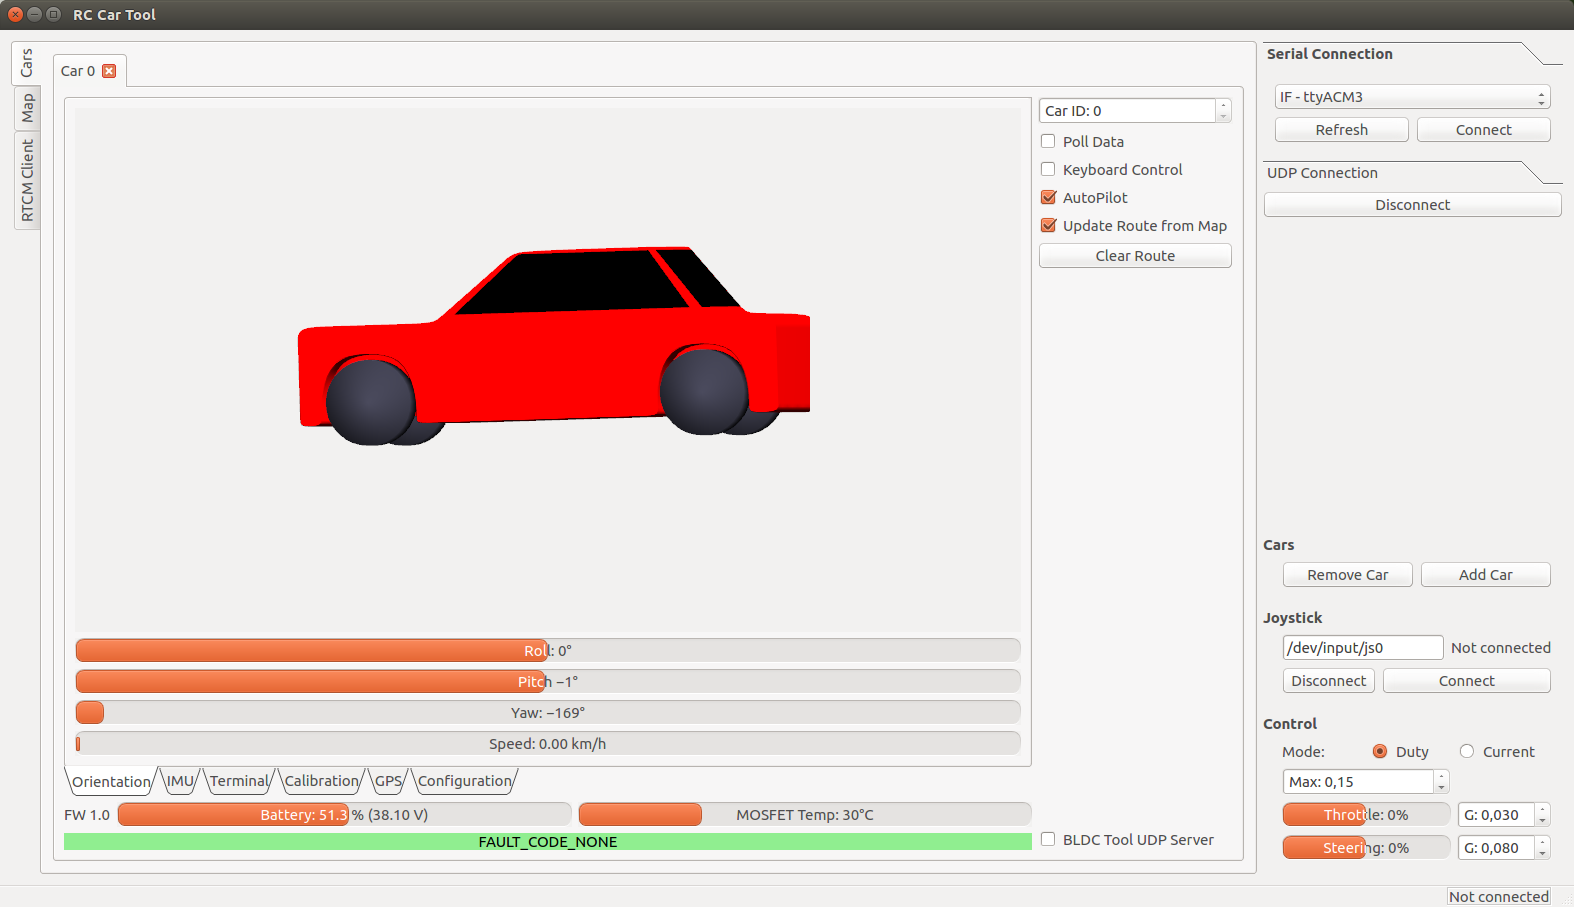
\includegraphics[width=11cm]{Figures/GUI/car_orientation.png}
\end{center}
\end{frame}

\begin{frame} 
\frametitle{The SP RC Car}
\framesubtitle{Linux Computer Block Diagram}
\begin{center}
	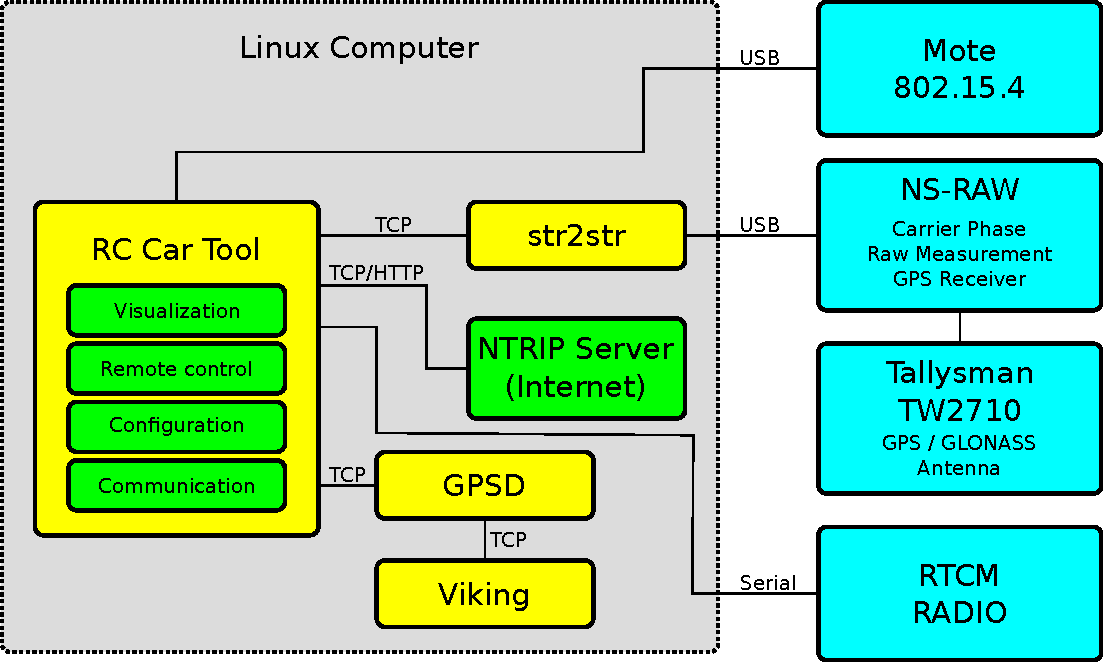
\includegraphics[width=10cm]{Figures/linux_diagram.pdf}
\end{center}
\end{frame}

\begin{frame} 
\frametitle{The SP RC Car}
\framesubtitle{RC Car Tool - IMU raw data}
\begin{center}
	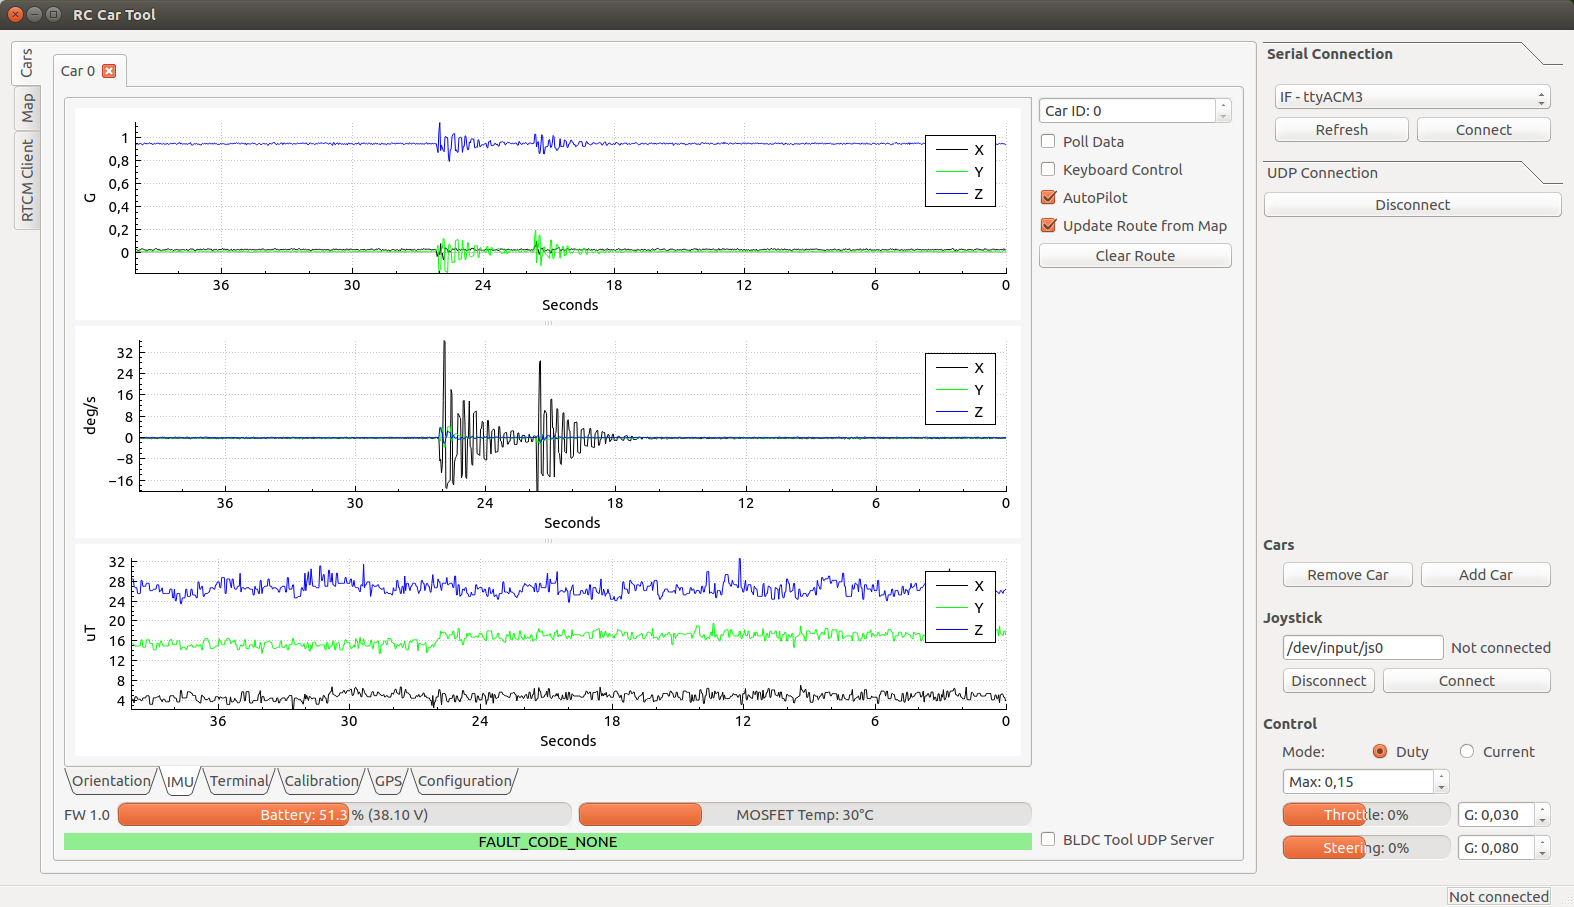
\includegraphics[width=11cm]{Figures/GUI/car_imu.png}
\end{center}
\end{frame}

\begin{frame} 
\frametitle{The SP RC Car}
\framesubtitle{RC Car Tool - Terminal}
\begin{center}
	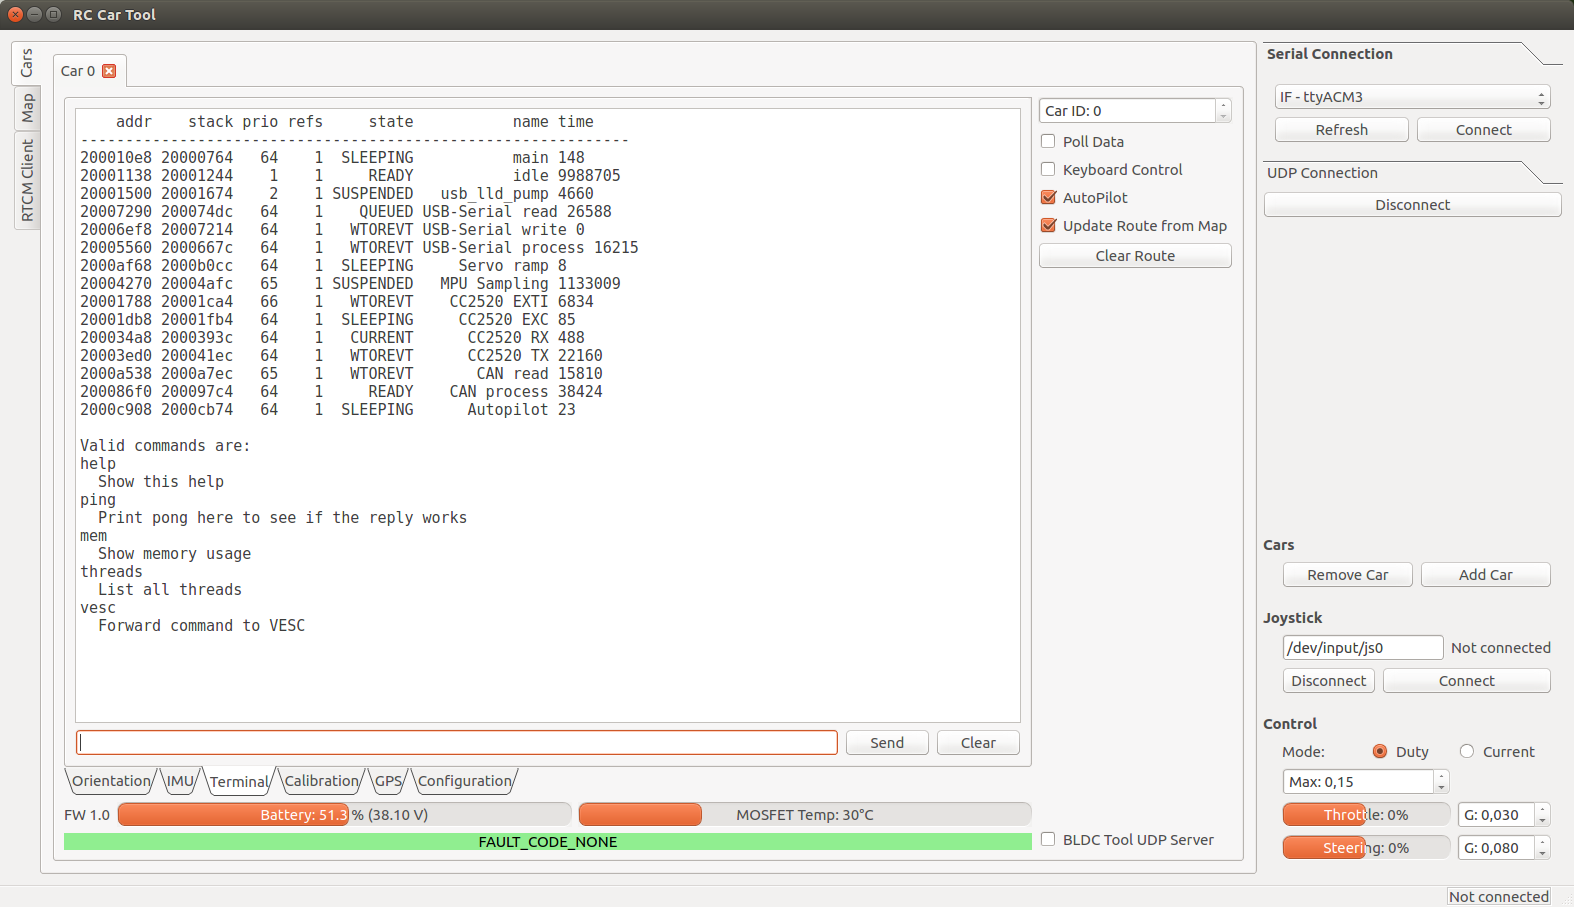
\includegraphics[width=11cm]{Figures/GUI/car_terminal.png}
\end{center}
\end{frame}

\begin{frame} 
\frametitle{The SP RC Car}
\framesubtitle{RC Car Tool - GPS Data}
\begin{center}
	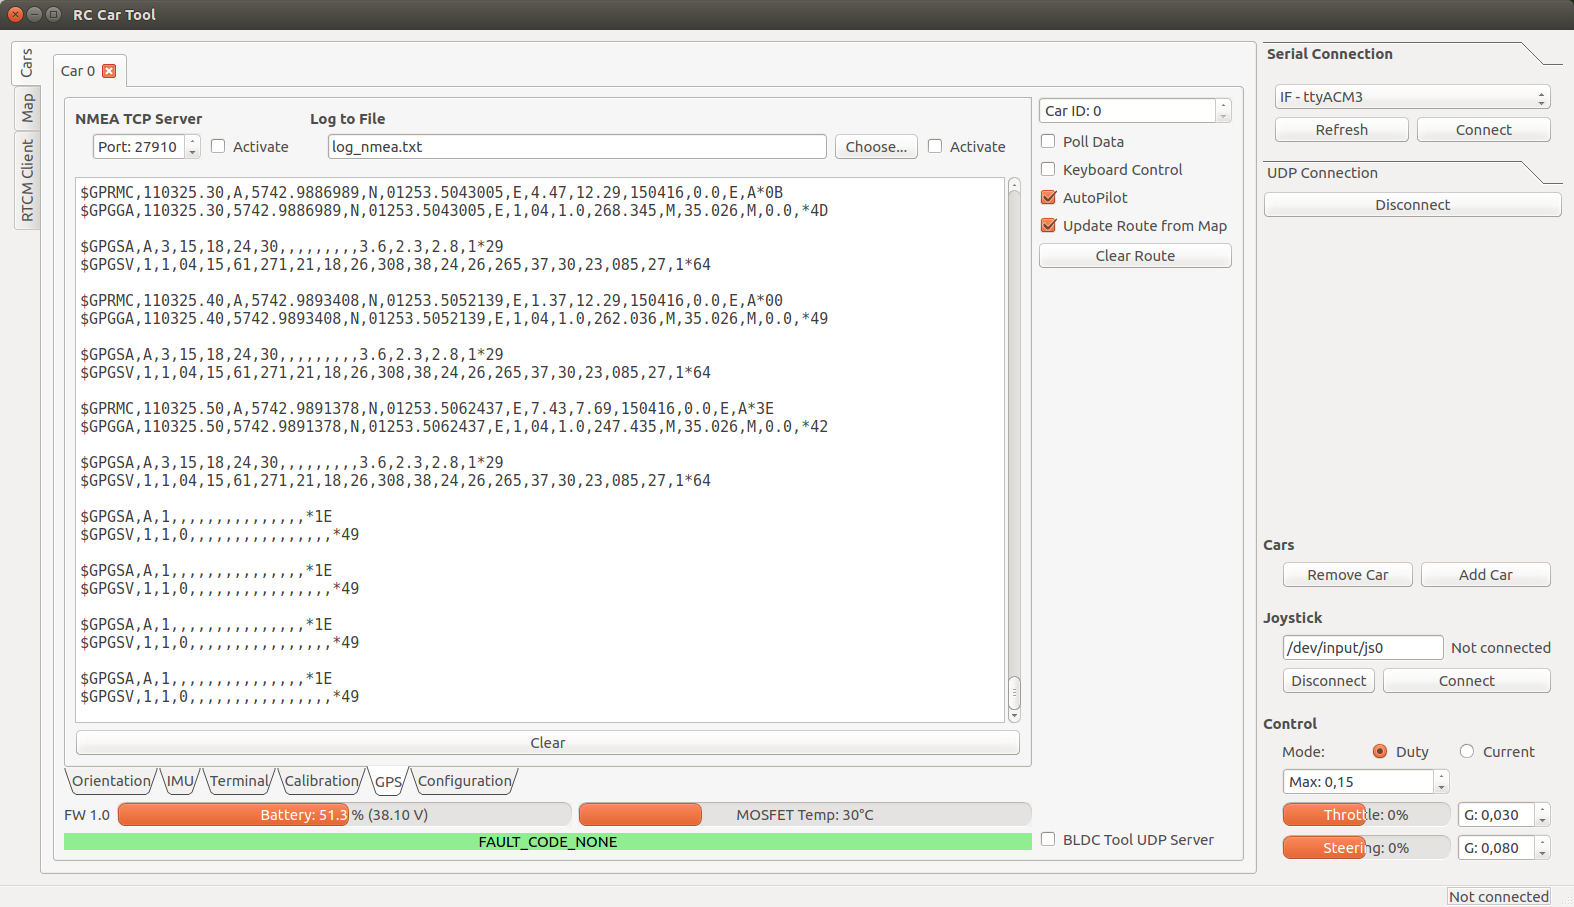
\includegraphics[width=11cm]{Figures/GUI/car_gps.png}
\end{center}
\end{frame}

\begin{frame} 
\frametitle{The SP RC Car}
\framesubtitle{RC Car Tool - Configuration}
\begin{center}
	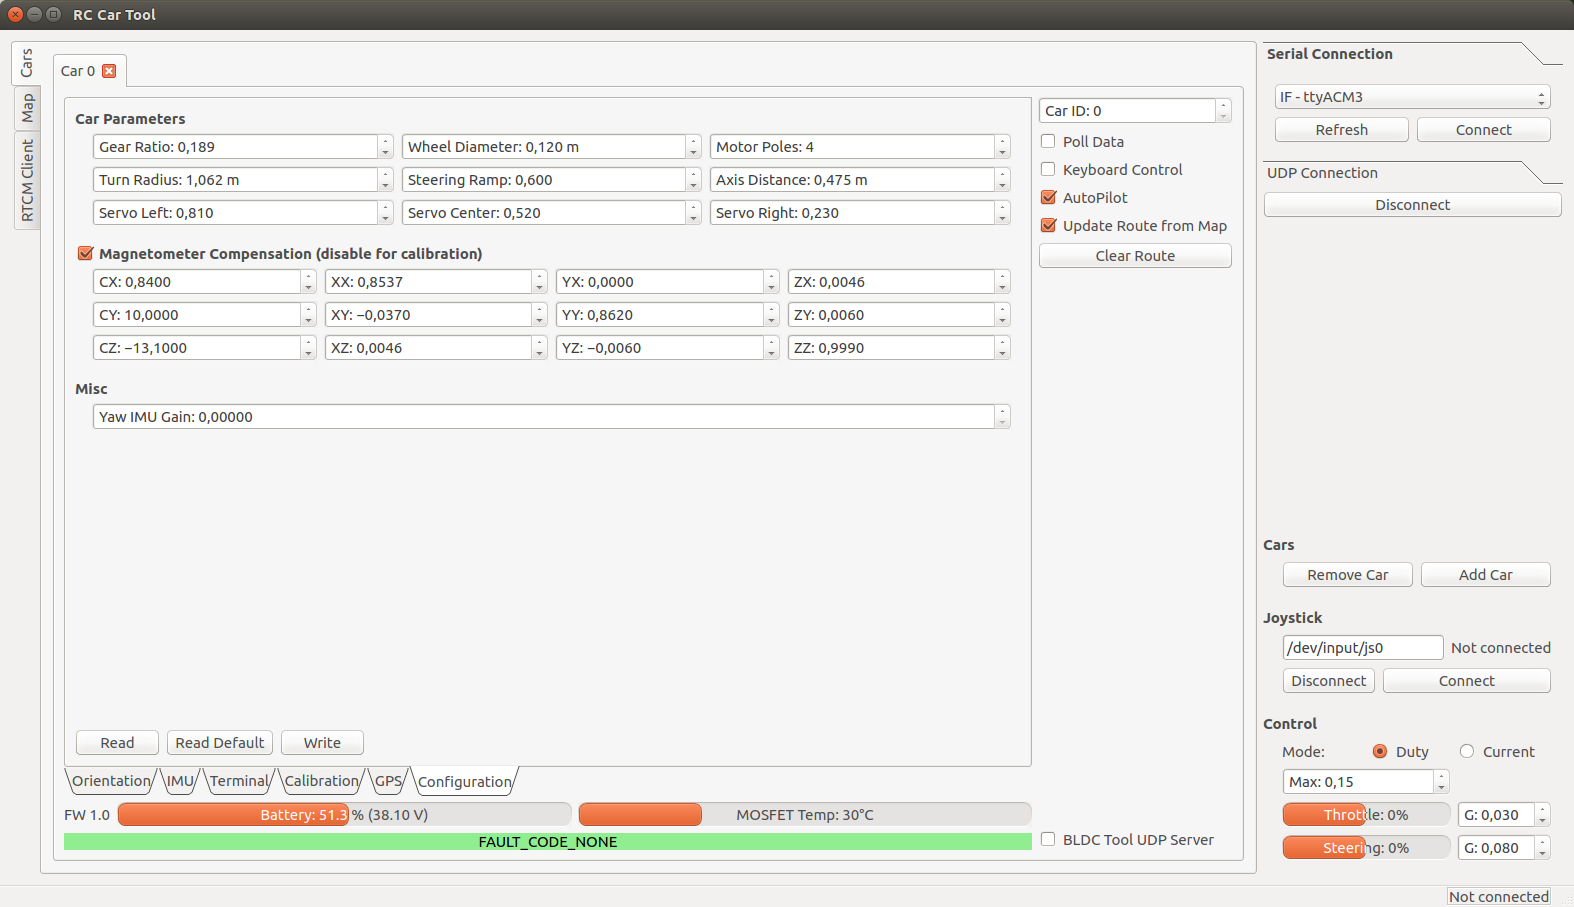
\includegraphics[width=11cm]{Figures/GUI/car_config.png}
\end{center}
\end{frame}

\begin{frame} 
\frametitle{The SP RC Car}
\framesubtitle{RC Car Tool - RTCM correction data}
\begin{center}
	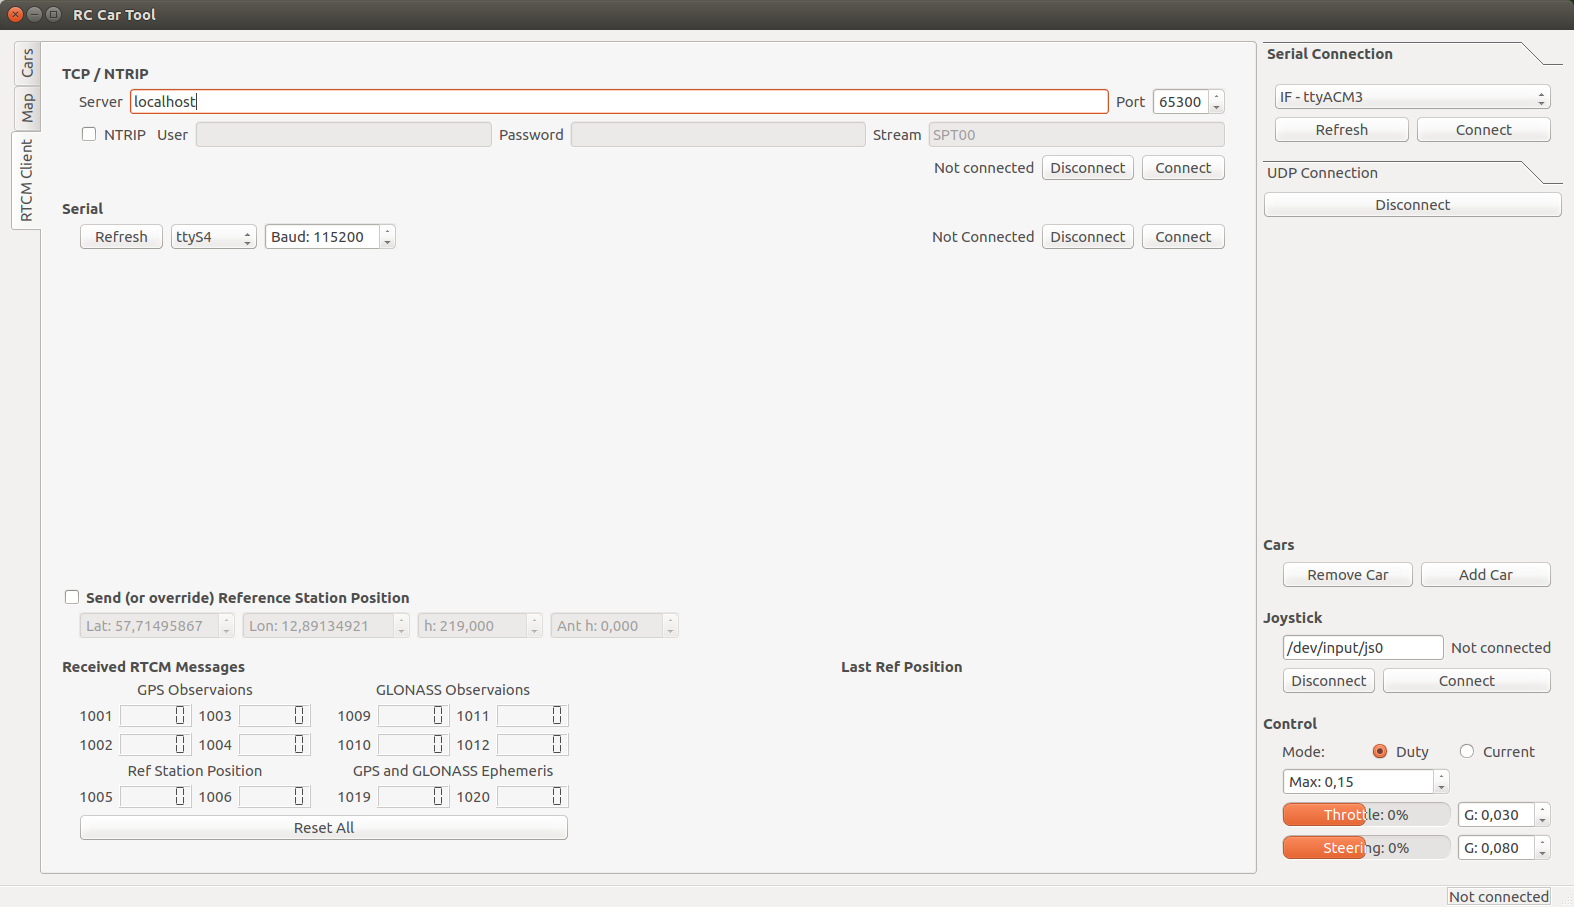
\includegraphics[width=11cm]{Figures/GUI/car_rtcm.png}
\end{center}
\end{frame}

\begin{frame} 
\frametitle{The SP RC Car}
\framesubtitle{RC Car Tool - Real-time plot and track editor for the autopilot}
\begin{center}
	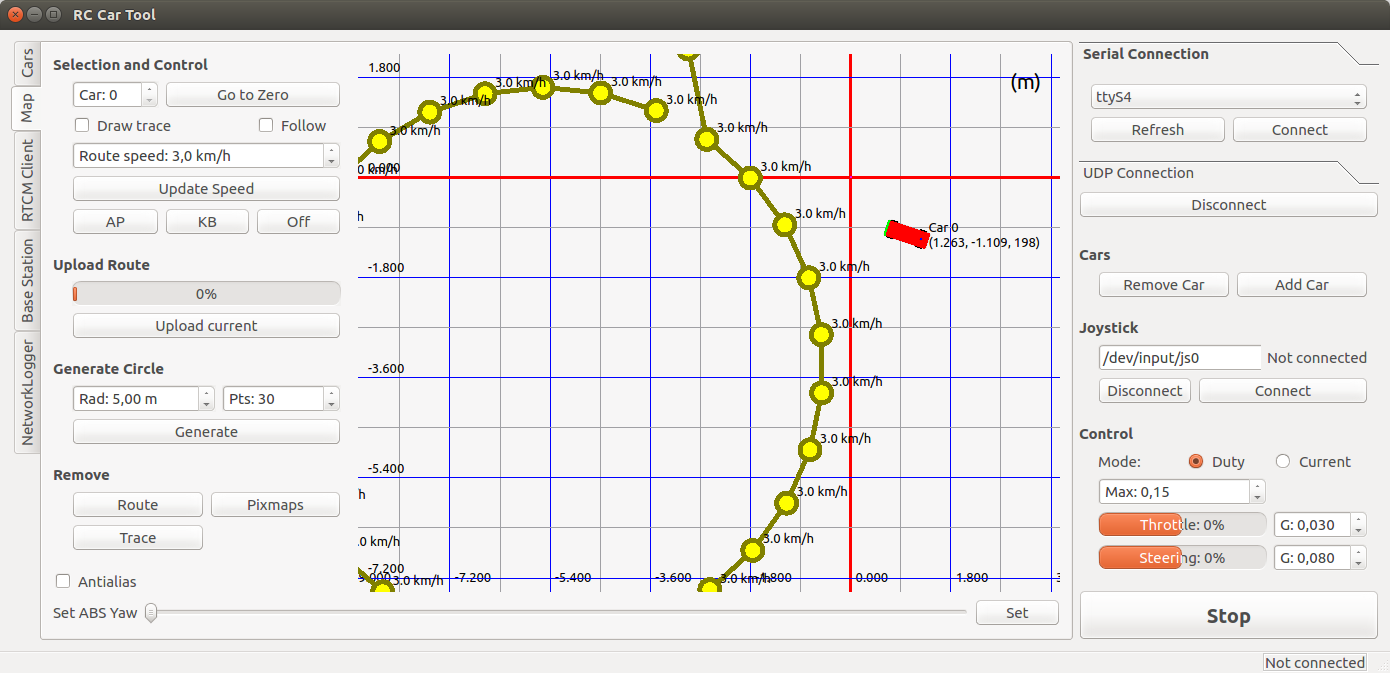
\includegraphics[width=11cm]{Figures/GUI/car_map.png}
\end{center}
\end{frame}

\spEndFrame

\end{document}